% \subsection{Wasserstein training with one-hot target}



% The one-hot encoding is a typical setting for multi-class one-label dataset. The distribution of a target label probability is ${\rm\textbf{t}}=\delta_{j,j^*}$, where $j^*$ is the ground truth class, $\delta_{j,j^*}$ is a Dirac delta, which equals to 1 for $j=j^*$\footnote{\noindent We use $i,j$ interlaced for ${\rm \textbf{s}}$ and ${\rm \textbf{t}}$, since they index the same group of positions in a circle.}, and $0$ otherwise. 

% \begin{figure}[t]
% \centering
% \begin{tabular}{cc}
% 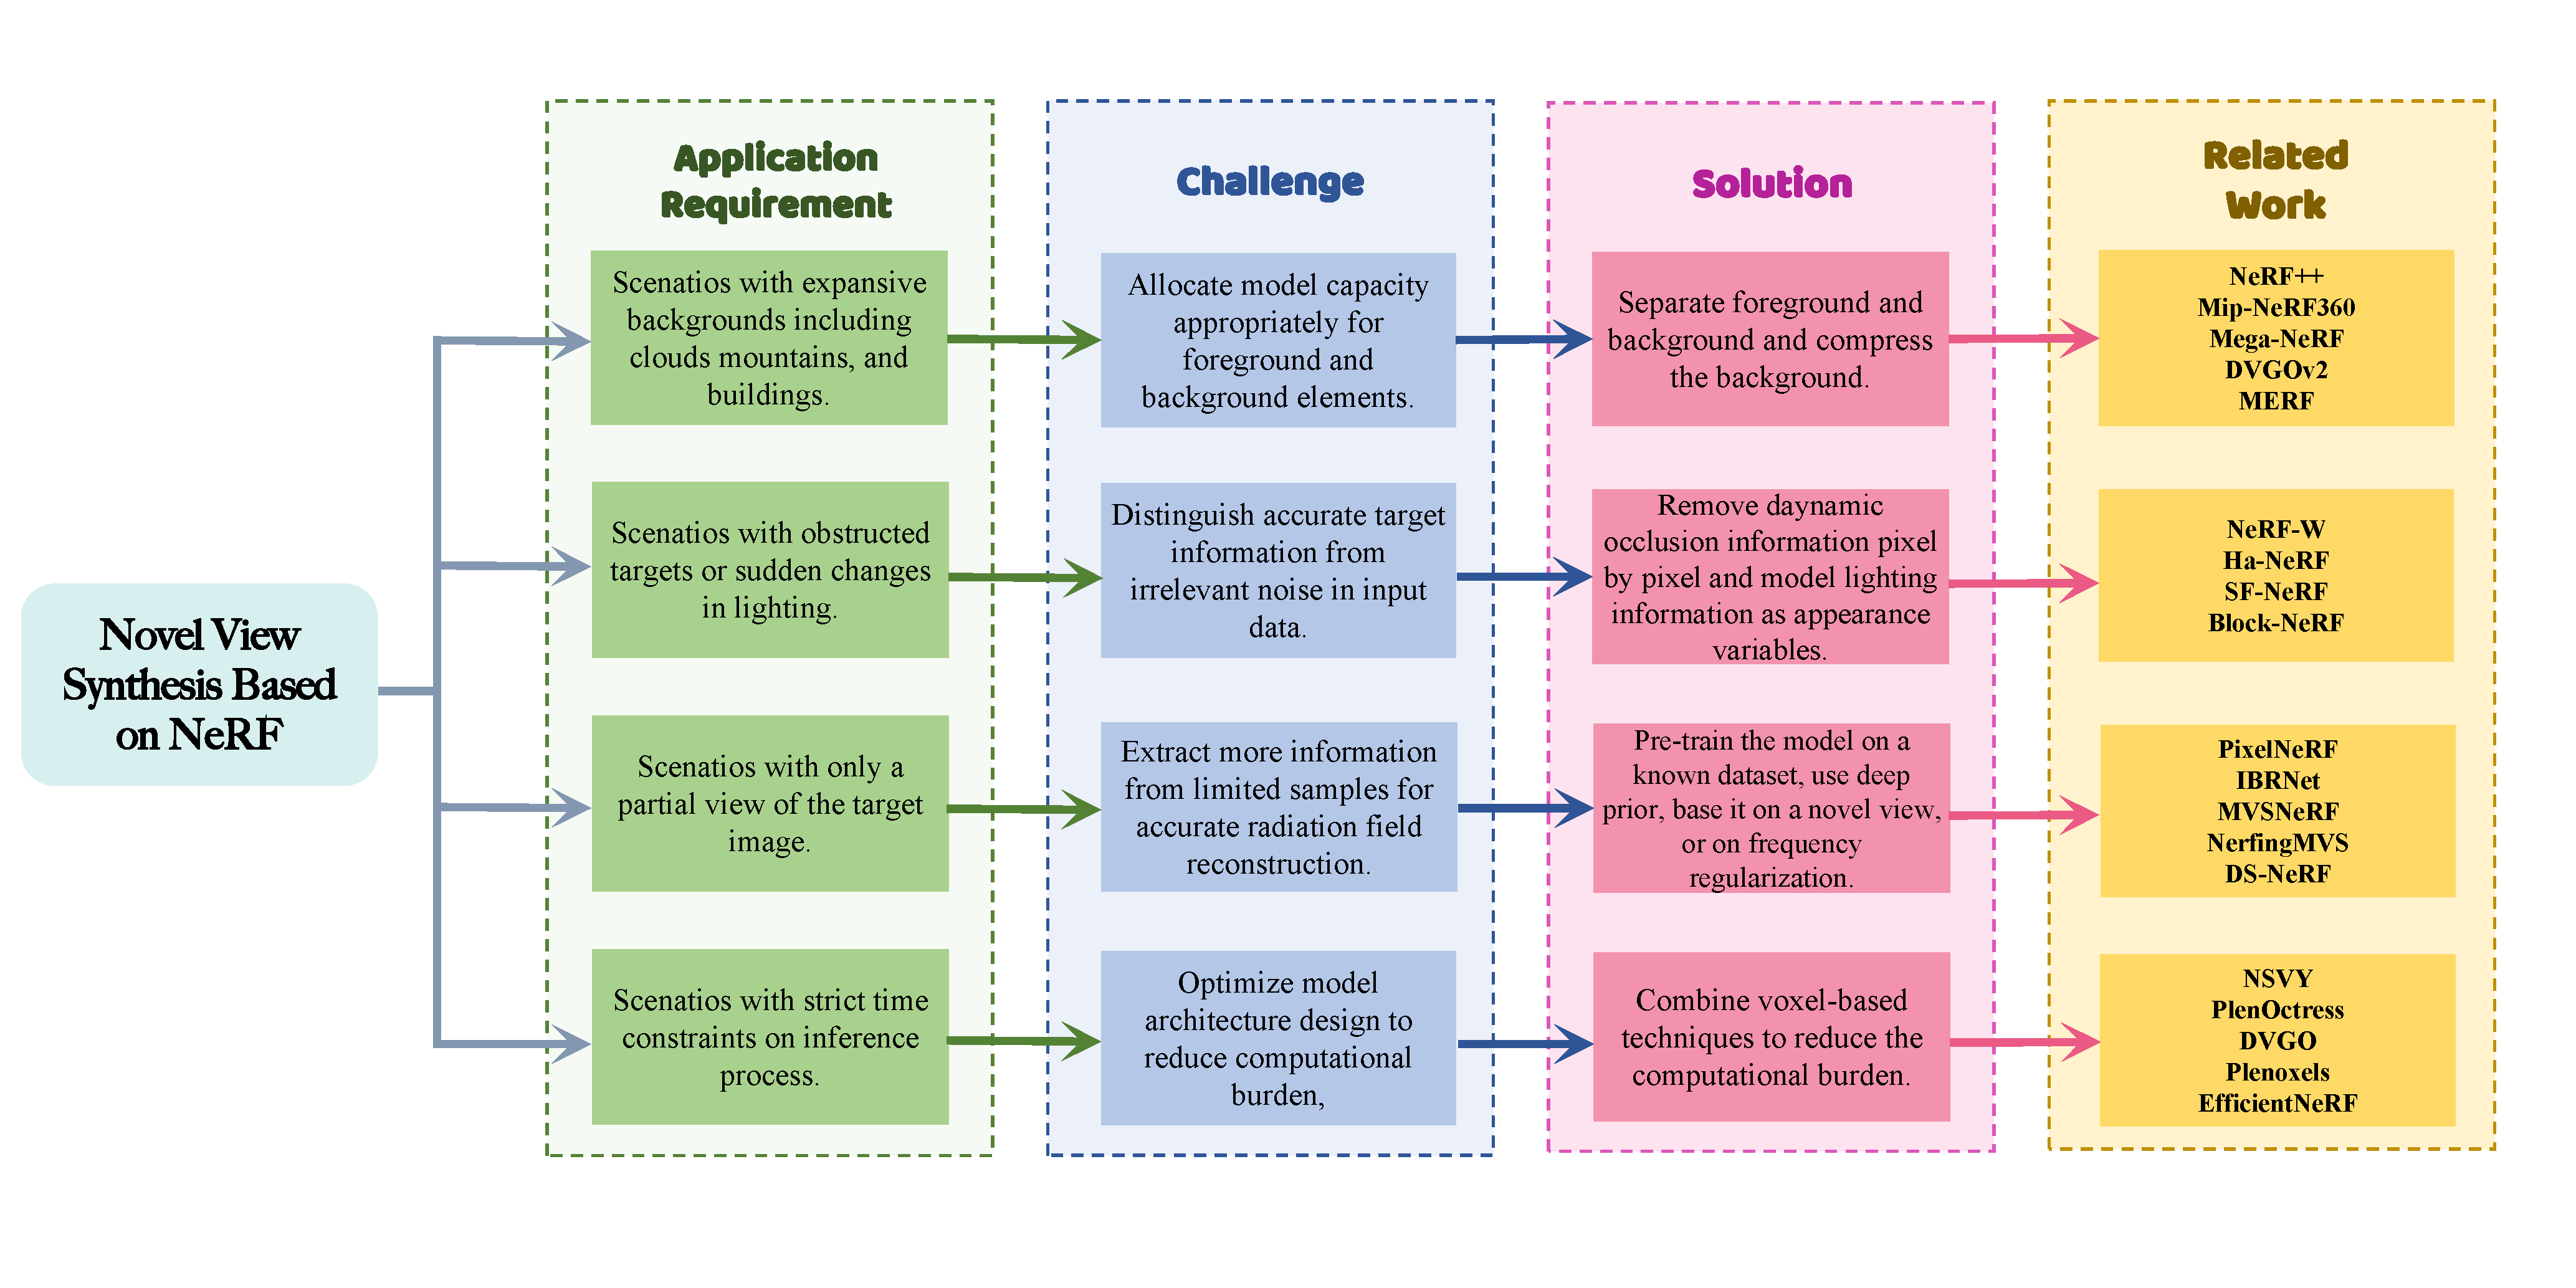
\includegraphics[height=6.8cm]{fig/NeRF.pdf}&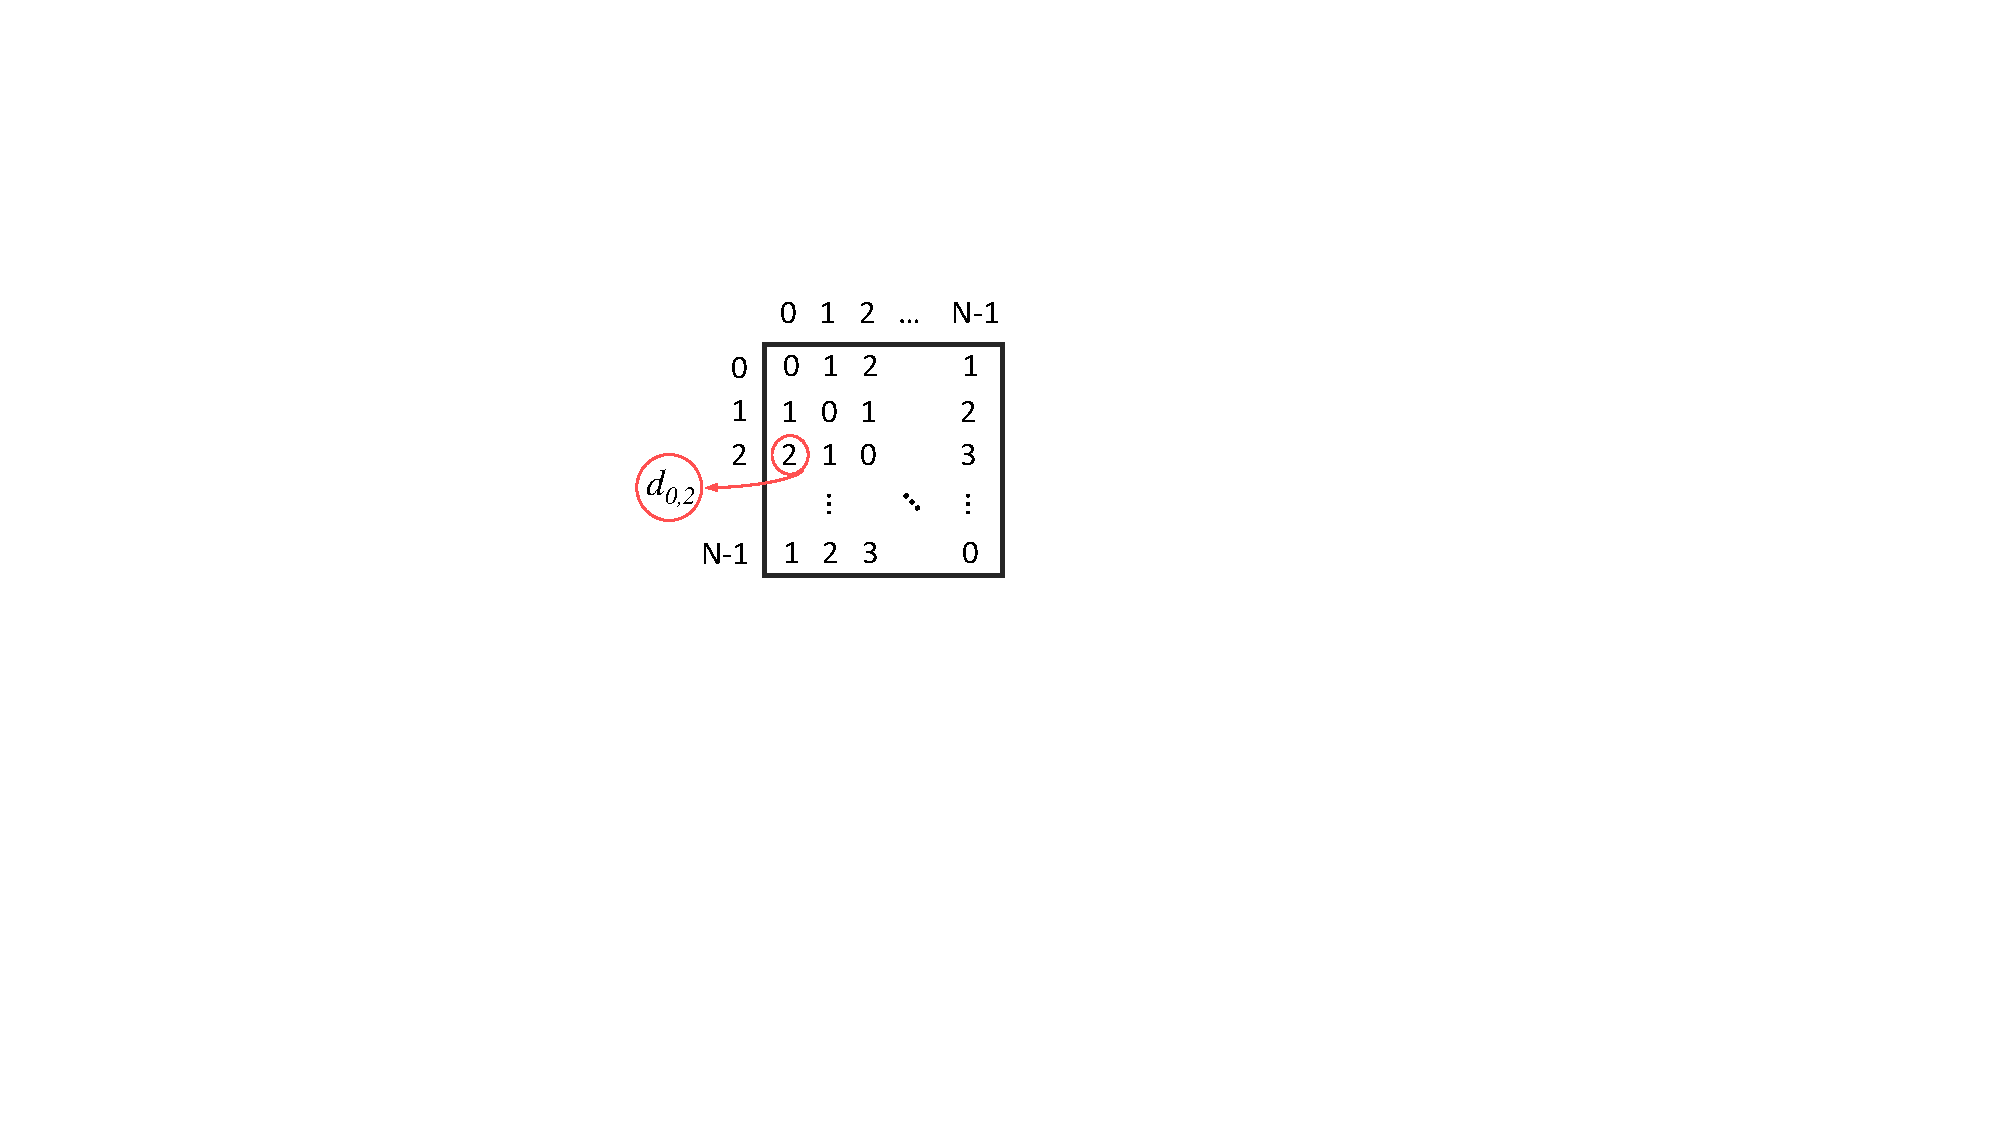
\includegraphics[height=2.8cm]{fig//fig2_2.pdf}
% \end{tabular}
% \caption{Left: The only possible transport plan in one-hot target case. Right: the ground matrix using arc length as ground metric.}
% \label{fig:2}
% \end{figure} 

% \noindent\textbf{Theorem 1.} \textit{Assume that} $\sum_{j=0}^{N-1}t_j=\sum_{i=0}^{N-1}s_i$, \textit{and} ${\rm{\textbf{t}}}$ \textit{is a one-hot distribution with} $t_{j^*}=1 ($or $\sum_{i=0}^{N-1}s_i)$\footnote{We note that softmax cannot strictly guarantee the sum of its outputs to be 1 considering the rounding operation. However, the difference of setting $t_{j^*}$ to $1$ or $\sum_{i=0}^{N-1}s_i)$ is not significant in our experiments using the typical format of softmax output which is accurate to 8 decimal places.}, \textit{there is only one feasible optimal transport plan.} 



% According to the criteria of ${\rm\textbf{W}}$, all masses have to be transferred to the cluster of the ground truth label $j^*$, as illustrated in Fig. \ref{fig:2}. Then, the Wasserstein distance between softmax prediction {\rm{\textbf{s}}} and one-hot target {\rm{\textbf{t}}} degenerates to\begin{equation}
% \mathcal{L}_{{\rm\textbf{D}}_{i,j}^{f}}({\rm{\textbf{s},\textbf{t}}})=\sum_{i=0}^{N-1} s_i f(d_{i,j^*}) \label{con:df}
% \end{equation} where ${\rm\textbf{D}}_{i,j}^f=f(d_{i,j})$. Practically, $f$ can be an increasing function proper, $e.g., p^{th}$ power of $d_{i,j}$ and Huber function. The exact solution of Eq. \eqref{con:df} can be computed with a complexity of $\mathcal{O}(N)$. The ground metric term $f(d_{i,j^*})$ works as the weights $w.r.t.$ $s_i$, which takes all classes into account following a soft attention scheme \cite{liu2018dependency,liu2019dependency,liu2019permutation}. It explicitly encourages the probabilities distributing on the neighboring classes of $j^*$. Since each $s_i$ is a function of the network parameters, differentiating $\mathcal{L}_{{\rm\textbf{D}}_{i,j}^{f}} w.r.t.$ network parameters yields $\sum_{i=0}^{N-1}s_i'f(d_{i,j^*})$.    



% In contrast, the cross-entropy loss in one-hot setting can be formulated as $-1{\rm log}s_{j^*}$, which only considers a single class prediction like the hard attention scheme \cite{liu2018dependency,liu2019dependency,liu2019permutation}, that usually loses too much information. Similarly, the regression loss using softmax prediction could be $f(d_{i^*,j^*})$, where $i^*$ is the class with maximum prediction probability.


% In addition to the predefined ground metric, we also propose to learn ${\rm\textbf{D}}$ adaptively along with our training following an alternative optimization scheme \cite{liu2018joint}.

% \noindent\textbf{Step 1:} Fixing ground matrix ${\rm\textbf{D}}$ to compute $\mathcal{L}_{{\rm\textbf{D}}_{i,j}}({\rm{\textbf{s},\textbf{t}}})$ and updating the network parameters.

% \noindent\textbf{Step 2:} Fixing network parameters and postprocessing ${\rm\textbf{D}}$ using the feature-level $\ell_1$ distances between different poses.

% We use the normalized second-to-last layer neural response in this round as feature vector, since there is no subsequent non-linearities. Therefore, it is meaningful to average the feature vectors in each pose class to compute their centroid and reconstruct ${{\rm\textbf{D}}_{i,j}}$ using the $\ell_1$ distances between these centroids $\overline{d}_{i,j}$. To avoid the model collapse, we construct the ${{\rm\textbf{D}}_{i,j}=\frac{1}{1+\alpha}\left\{f(\overline{d}_{i,j})+\alpha f(d_{i,j})\right\}}$ in each round, and decrease $\alpha$ from 10 to 0 gradually in the training.   
 

 







